% Created by tikzDevice version 0.12.6 on 2025-02-15 05:56:28
% !TEX encoding = UTF-8 Unicode
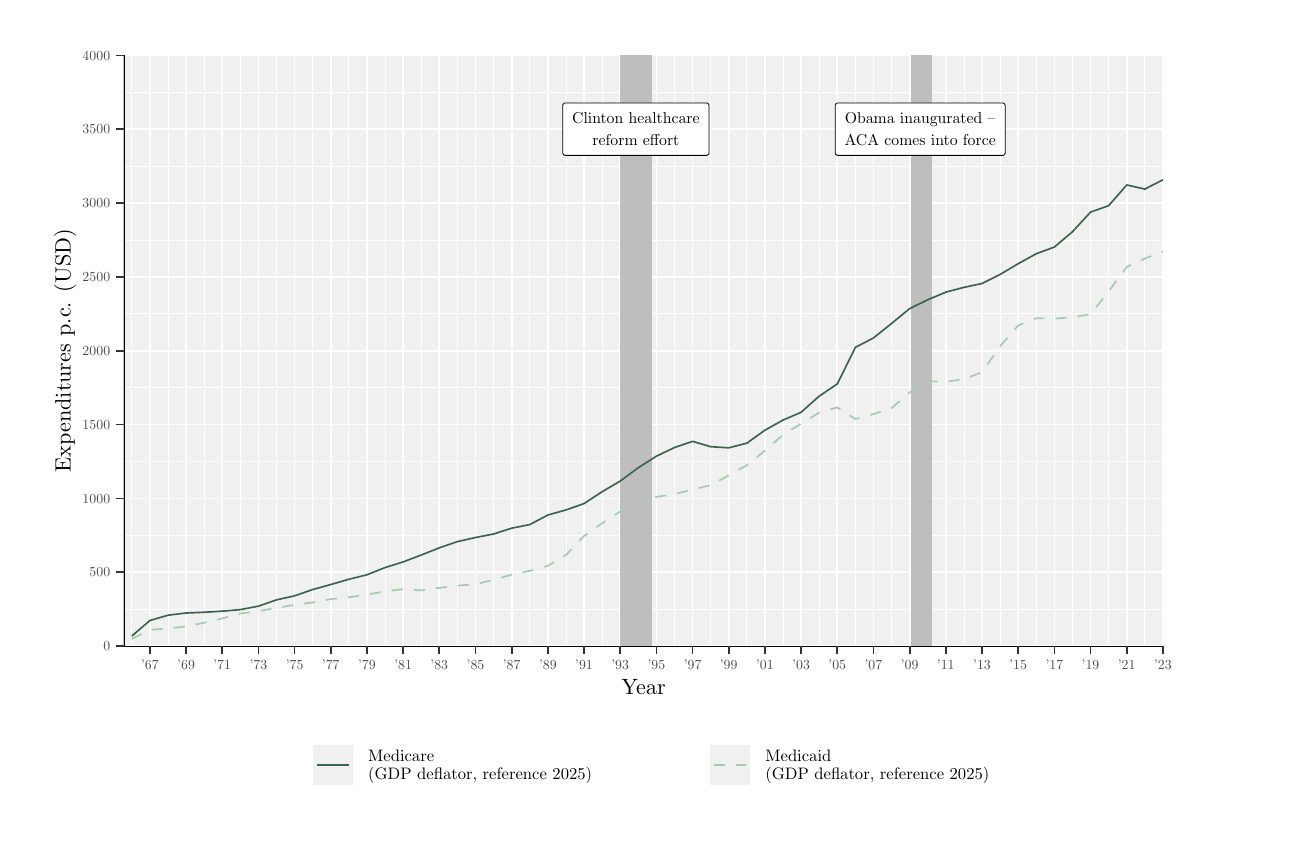
\begin{tikzpicture}[x=1pt,y=1pt]
\definecolor{fillColor}{RGB}{255,255,255}
\path[use as bounding box,fill=fillColor,fill opacity=0.00] (0,0) rectangle (455.30,289.08);
\begin{scope}
\path[clip] (  0.00,  0.00) rectangle (455.30,289.08);
\definecolor{drawColor}{RGB}{255,255,255}
\definecolor{fillColor}{RGB}{255,255,255}

\path[draw=drawColor,line width= 0.6pt,line join=round,line cap=round,fill=fillColor] (  0.00,  0.00) rectangle (455.30,289.08);
\end{scope}
\begin{scope}
\path[clip] (  0.00,  0.00) rectangle (455.30,289.08);
\definecolor{fillColor}{gray}{0.94}

\path[fill=fillColor] ( 34.76, 65.63) rectangle (410.30,279.08);
\definecolor{drawColor}{RGB}{255,255,255}

\path[draw=drawColor,line width= 0.3pt,line join=round] ( 34.76, 78.97) --
	(410.30, 78.97);

\path[draw=drawColor,line width= 0.3pt,line join=round] ( 34.76,105.66) --
	(410.30,105.66);

\path[draw=drawColor,line width= 0.3pt,line join=round] ( 34.76,132.34) --
	(410.30,132.34);

\path[draw=drawColor,line width= 0.3pt,line join=round] ( 34.76,159.02) --
	(410.30,159.02);

\path[draw=drawColor,line width= 0.3pt,line join=round] ( 34.76,185.70) --
	(410.30,185.70);

\path[draw=drawColor,line width= 0.3pt,line join=round] ( 34.76,212.38) --
	(410.30,212.38);

\path[draw=drawColor,line width= 0.3pt,line join=round] ( 34.76,239.06) --
	(410.30,239.06);

\path[draw=drawColor,line width= 0.3pt,line join=round] ( 34.76,265.74) --
	(410.30,265.74);

\path[draw=drawColor,line width= 0.3pt,line join=round] ( 37.63, 65.63) --
	( 37.63,279.08);

\path[draw=drawColor,line width= 0.3pt,line join=round] ( 50.70, 65.63) --
	( 50.70,279.08);

\path[draw=drawColor,line width= 0.3pt,line join=round] ( 63.77, 65.63) --
	( 63.77,279.08);

\path[draw=drawColor,line width= 0.3pt,line join=round] ( 76.85, 65.63) --
	( 76.85,279.08);

\path[draw=drawColor,line width= 0.3pt,line join=round] ( 89.92, 65.63) --
	( 89.92,279.08);

\path[draw=drawColor,line width= 0.3pt,line join=round] (102.99, 65.63) --
	(102.99,279.08);

\path[draw=drawColor,line width= 0.3pt,line join=round] (116.07, 65.63) --
	(116.07,279.08);

\path[draw=drawColor,line width= 0.3pt,line join=round] (129.14, 65.63) --
	(129.14,279.08);

\path[draw=drawColor,line width= 0.3pt,line join=round] (142.21, 65.63) --
	(142.21,279.08);

\path[draw=drawColor,line width= 0.3pt,line join=round] (155.29, 65.63) --
	(155.29,279.08);

\path[draw=drawColor,line width= 0.3pt,line join=round] (168.36, 65.63) --
	(168.36,279.08);

\path[draw=drawColor,line width= 0.3pt,line join=round] (181.43, 65.63) --
	(181.43,279.08);

\path[draw=drawColor,line width= 0.3pt,line join=round] (194.51, 65.63) --
	(194.51,279.08);

\path[draw=drawColor,line width= 0.3pt,line join=round] (207.58, 65.63) --
	(207.58,279.08);

\path[draw=drawColor,line width= 0.3pt,line join=round] (220.65, 65.63) --
	(220.65,279.08);

\path[draw=drawColor,line width= 0.3pt,line join=round] (233.73, 65.63) --
	(233.73,279.08);

\path[draw=drawColor,line width= 0.3pt,line join=round] (246.80, 65.63) --
	(246.80,279.08);

\path[draw=drawColor,line width= 0.3pt,line join=round] (259.87, 65.63) --
	(259.87,279.08);

\path[draw=drawColor,line width= 0.3pt,line join=round] (272.95, 65.63) --
	(272.95,279.08);

\path[draw=drawColor,line width= 0.3pt,line join=round] (286.02, 65.63) --
	(286.02,279.08);

\path[draw=drawColor,line width= 0.3pt,line join=round] (299.09, 65.63) --
	(299.09,279.08);

\path[draw=drawColor,line width= 0.3pt,line join=round] (312.17, 65.63) --
	(312.17,279.08);

\path[draw=drawColor,line width= 0.3pt,line join=round] (325.24, 65.63) --
	(325.24,279.08);

\path[draw=drawColor,line width= 0.3pt,line join=round] (338.31, 65.63) --
	(338.31,279.08);

\path[draw=drawColor,line width= 0.3pt,line join=round] (351.39, 65.63) --
	(351.39,279.08);

\path[draw=drawColor,line width= 0.3pt,line join=round] (364.46, 65.63) --
	(364.46,279.08);

\path[draw=drawColor,line width= 0.3pt,line join=round] (377.53, 65.63) --
	(377.53,279.08);

\path[draw=drawColor,line width= 0.3pt,line join=round] (390.61, 65.63) --
	(390.61,279.08);

\path[draw=drawColor,line width= 0.3pt,line join=round] (403.68, 65.63) --
	(403.68,279.08);

\path[draw=drawColor,line width= 0.6pt,line join=round] ( 34.76, 65.63) --
	(410.30, 65.63);

\path[draw=drawColor,line width= 0.6pt,line join=round] ( 34.76, 92.32) --
	(410.30, 92.32);

\path[draw=drawColor,line width= 0.6pt,line join=round] ( 34.76,119.00) --
	(410.30,119.00);

\path[draw=drawColor,line width= 0.6pt,line join=round] ( 34.76,145.68) --
	(410.30,145.68);

\path[draw=drawColor,line width= 0.6pt,line join=round] ( 34.76,172.36) --
	(410.30,172.36);

\path[draw=drawColor,line width= 0.6pt,line join=round] ( 34.76,199.04) --
	(410.30,199.04);

\path[draw=drawColor,line width= 0.6pt,line join=round] ( 34.76,225.72) --
	(410.30,225.72);

\path[draw=drawColor,line width= 0.6pt,line join=round] ( 34.76,252.40) --
	(410.30,252.40);

\path[draw=drawColor,line width= 0.6pt,line join=round] ( 34.76,279.08) --
	(410.30,279.08);

\path[draw=drawColor,line width= 0.6pt,line join=round] ( 44.16, 65.63) --
	( 44.16,279.08);

\path[draw=drawColor,line width= 0.6pt,line join=round] ( 57.24, 65.63) --
	( 57.24,279.08);

\path[draw=drawColor,line width= 0.6pt,line join=round] ( 70.30, 65.63) --
	( 70.30,279.08);

\path[draw=drawColor,line width= 0.6pt,line join=round] ( 83.39, 65.63) --
	( 83.39,279.08);

\path[draw=drawColor,line width= 0.6pt,line join=round] ( 96.45, 65.63) --
	( 96.45,279.08);

\path[draw=drawColor,line width= 0.6pt,line join=round] (109.53, 65.63) --
	(109.53,279.08);

\path[draw=drawColor,line width= 0.6pt,line join=round] (122.60, 65.63) --
	(122.60,279.08);

\path[draw=drawColor,line width= 0.6pt,line join=round] (135.68, 65.63) --
	(135.68,279.08);

\path[draw=drawColor,line width= 0.6pt,line join=round] (148.74, 65.63) --
	(148.74,279.08);

\path[draw=drawColor,line width= 0.6pt,line join=round] (161.83, 65.63) --
	(161.83,279.08);

\path[draw=drawColor,line width= 0.6pt,line join=round] (174.89, 65.63) --
	(174.89,279.08);

\path[draw=drawColor,line width= 0.6pt,line join=round] (187.97, 65.63) --
	(187.97,279.08);

\path[draw=drawColor,line width= 0.6pt,line join=round] (201.04, 65.63) --
	(201.04,279.08);

\path[draw=drawColor,line width= 0.6pt,line join=round] (214.12, 65.63) --
	(214.12,279.08);

\path[draw=drawColor,line width= 0.6pt,line join=round] (227.18, 65.63) --
	(227.18,279.08);

\path[draw=drawColor,line width= 0.6pt,line join=round] (240.27, 65.63) --
	(240.27,279.08);

\path[draw=drawColor,line width= 0.6pt,line join=round] (253.33, 65.63) --
	(253.33,279.08);

\path[draw=drawColor,line width= 0.6pt,line join=round] (266.41, 65.63) --
	(266.41,279.08);

\path[draw=drawColor,line width= 0.6pt,line join=round] (279.48, 65.63) --
	(279.48,279.08);

\path[draw=drawColor,line width= 0.6pt,line join=round] (292.56, 65.63) --
	(292.56,279.08);

\path[draw=drawColor,line width= 0.6pt,line join=round] (305.62, 65.63) --
	(305.62,279.08);

\path[draw=drawColor,line width= 0.6pt,line join=round] (318.71, 65.63) --
	(318.71,279.08);

\path[draw=drawColor,line width= 0.6pt,line join=round] (331.77, 65.63) --
	(331.77,279.08);

\path[draw=drawColor,line width= 0.6pt,line join=round] (344.85, 65.63) --
	(344.85,279.08);

\path[draw=drawColor,line width= 0.6pt,line join=round] (357.92, 65.63) --
	(357.92,279.08);

\path[draw=drawColor,line width= 0.6pt,line join=round] (371.00, 65.63) --
	(371.00,279.08);

\path[draw=drawColor,line width= 0.6pt,line join=round] (384.06, 65.63) --
	(384.06,279.08);

\path[draw=drawColor,line width= 0.6pt,line join=round] (397.15, 65.63) --
	(397.15,279.08);

\path[draw=drawColor,line width= 0.6pt,line join=round] (410.21, 65.63) --
	(410.21,279.08);
\definecolor{fillColor}{RGB}{190,190,190}

\path[fill=fillColor,fill opacity=0.01] (214.12, 65.63) rectangle (225.45,279.08);

\path[fill=fillColor,fill opacity=0.01] (214.12, 65.63) rectangle (225.45,279.08);

\path[fill=fillColor,fill opacity=0.01] (214.12, 65.63) rectangle (225.45,279.08);

\path[fill=fillColor,fill opacity=0.01] (214.12, 65.63) rectangle (225.45,279.08);

\path[fill=fillColor,fill opacity=0.01] (214.12, 65.63) rectangle (225.45,279.08);

\path[fill=fillColor,fill opacity=0.01] (214.12, 65.63) rectangle (225.45,279.08);

\path[fill=fillColor,fill opacity=0.01] (214.12, 65.63) rectangle (225.45,279.08);

\path[fill=fillColor,fill opacity=0.01] (214.12, 65.63) rectangle (225.45,279.08);

\path[fill=fillColor,fill opacity=0.01] (214.12, 65.63) rectangle (225.45,279.08);

\path[fill=fillColor,fill opacity=0.01] (214.12, 65.63) rectangle (225.45,279.08);

\path[fill=fillColor,fill opacity=0.01] (214.12, 65.63) rectangle (225.45,279.08);

\path[fill=fillColor,fill opacity=0.01] (214.12, 65.63) rectangle (225.45,279.08);

\path[fill=fillColor,fill opacity=0.01] (214.12, 65.63) rectangle (225.45,279.08);

\path[fill=fillColor,fill opacity=0.01] (214.12, 65.63) rectangle (225.45,279.08);

\path[fill=fillColor,fill opacity=0.01] (214.12, 65.63) rectangle (225.45,279.08);

\path[fill=fillColor,fill opacity=0.01] (214.12, 65.63) rectangle (225.45,279.08);

\path[fill=fillColor,fill opacity=0.01] (214.12, 65.63) rectangle (225.45,279.08);

\path[fill=fillColor,fill opacity=0.01] (214.12, 65.63) rectangle (225.45,279.08);

\path[fill=fillColor,fill opacity=0.01] (214.12, 65.63) rectangle (225.45,279.08);

\path[fill=fillColor,fill opacity=0.01] (214.12, 65.63) rectangle (225.45,279.08);

\path[fill=fillColor,fill opacity=0.01] (214.12, 65.63) rectangle (225.45,279.08);

\path[fill=fillColor,fill opacity=0.01] (214.12, 65.63) rectangle (225.45,279.08);

\path[fill=fillColor,fill opacity=0.01] (214.12, 65.63) rectangle (225.45,279.08);

\path[fill=fillColor,fill opacity=0.01] (214.12, 65.63) rectangle (225.45,279.08);

\path[fill=fillColor,fill opacity=0.01] (214.12, 65.63) rectangle (225.45,279.08);

\path[fill=fillColor,fill opacity=0.01] (214.12, 65.63) rectangle (225.45,279.08);

\path[fill=fillColor,fill opacity=0.01] (214.12, 65.63) rectangle (225.45,279.08);

\path[fill=fillColor,fill opacity=0.01] (214.12, 65.63) rectangle (225.45,279.08);

\path[fill=fillColor,fill opacity=0.01] (214.12, 65.63) rectangle (225.45,279.08);

\path[fill=fillColor,fill opacity=0.01] (214.12, 65.63) rectangle (225.45,279.08);

\path[fill=fillColor,fill opacity=0.01] (214.12, 65.63) rectangle (225.45,279.08);

\path[fill=fillColor,fill opacity=0.01] (214.12, 65.63) rectangle (225.45,279.08);

\path[fill=fillColor,fill opacity=0.01] (214.12, 65.63) rectangle (225.45,279.08);

\path[fill=fillColor,fill opacity=0.01] (214.12, 65.63) rectangle (225.45,279.08);

\path[fill=fillColor,fill opacity=0.01] (214.12, 65.63) rectangle (225.45,279.08);

\path[fill=fillColor,fill opacity=0.01] (214.12, 65.63) rectangle (225.45,279.08);

\path[fill=fillColor,fill opacity=0.01] (214.12, 65.63) rectangle (225.45,279.08);

\path[fill=fillColor,fill opacity=0.01] (214.12, 65.63) rectangle (225.45,279.08);

\path[fill=fillColor,fill opacity=0.01] (214.12, 65.63) rectangle (225.45,279.08);

\path[fill=fillColor,fill opacity=0.01] (214.12, 65.63) rectangle (225.45,279.08);

\path[fill=fillColor,fill opacity=0.01] (214.12, 65.63) rectangle (225.45,279.08);

\path[fill=fillColor,fill opacity=0.01] (214.12, 65.63) rectangle (225.45,279.08);

\path[fill=fillColor,fill opacity=0.01] (214.12, 65.63) rectangle (225.45,279.08);

\path[fill=fillColor,fill opacity=0.01] (214.12, 65.63) rectangle (225.45,279.08);

\path[fill=fillColor,fill opacity=0.01] (214.12, 65.63) rectangle (225.45,279.08);

\path[fill=fillColor,fill opacity=0.01] (214.12, 65.63) rectangle (225.45,279.08);

\path[fill=fillColor,fill opacity=0.01] (214.12, 65.63) rectangle (225.45,279.08);

\path[fill=fillColor,fill opacity=0.01] (214.12, 65.63) rectangle (225.45,279.08);

\path[fill=fillColor,fill opacity=0.01] (214.12, 65.63) rectangle (225.45,279.08);

\path[fill=fillColor,fill opacity=0.01] (214.12, 65.63) rectangle (225.45,279.08);

\path[fill=fillColor,fill opacity=0.01] (214.12, 65.63) rectangle (225.45,279.08);

\path[fill=fillColor,fill opacity=0.01] (214.12, 65.63) rectangle (225.45,279.08);

\path[fill=fillColor,fill opacity=0.01] (214.12, 65.63) rectangle (225.45,279.08);

\path[fill=fillColor,fill opacity=0.01] (214.12, 65.63) rectangle (225.45,279.08);

\path[fill=fillColor,fill opacity=0.01] (214.12, 65.63) rectangle (225.45,279.08);

\path[fill=fillColor,fill opacity=0.01] (214.12, 65.63) rectangle (225.45,279.08);

\path[fill=fillColor,fill opacity=0.01] (214.12, 65.63) rectangle (225.45,279.08);

\path[fill=fillColor,fill opacity=0.01] (214.12, 65.63) rectangle (225.45,279.08);

\path[fill=fillColor,fill opacity=0.01] (214.12, 65.63) rectangle (225.45,279.08);

\path[fill=fillColor,fill opacity=0.01] (214.12, 65.63) rectangle (225.45,279.08);

\path[fill=fillColor,fill opacity=0.01] (214.12, 65.63) rectangle (225.45,279.08);

\path[fill=fillColor,fill opacity=0.01] (214.12, 65.63) rectangle (225.45,279.08);

\path[fill=fillColor,fill opacity=0.01] (214.12, 65.63) rectangle (225.45,279.08);

\path[fill=fillColor,fill opacity=0.01] (214.12, 65.63) rectangle (225.45,279.08);

\path[fill=fillColor,fill opacity=0.01] (319.05, 65.63) rectangle (326.69,279.08);

\path[fill=fillColor,fill opacity=0.01] (319.05, 65.63) rectangle (326.69,279.08);

\path[fill=fillColor,fill opacity=0.01] (319.05, 65.63) rectangle (326.69,279.08);

\path[fill=fillColor,fill opacity=0.01] (319.05, 65.63) rectangle (326.69,279.08);

\path[fill=fillColor,fill opacity=0.01] (319.05, 65.63) rectangle (326.69,279.08);

\path[fill=fillColor,fill opacity=0.01] (319.05, 65.63) rectangle (326.69,279.08);

\path[fill=fillColor,fill opacity=0.01] (319.05, 65.63) rectangle (326.69,279.08);

\path[fill=fillColor,fill opacity=0.01] (319.05, 65.63) rectangle (326.69,279.08);

\path[fill=fillColor,fill opacity=0.01] (319.05, 65.63) rectangle (326.69,279.08);

\path[fill=fillColor,fill opacity=0.01] (319.05, 65.63) rectangle (326.69,279.08);

\path[fill=fillColor,fill opacity=0.01] (319.05, 65.63) rectangle (326.69,279.08);

\path[fill=fillColor,fill opacity=0.01] (319.05, 65.63) rectangle (326.69,279.08);

\path[fill=fillColor,fill opacity=0.01] (319.05, 65.63) rectangle (326.69,279.08);

\path[fill=fillColor,fill opacity=0.01] (319.05, 65.63) rectangle (326.69,279.08);

\path[fill=fillColor,fill opacity=0.01] (319.05, 65.63) rectangle (326.69,279.08);

\path[fill=fillColor,fill opacity=0.01] (319.05, 65.63) rectangle (326.69,279.08);

\path[fill=fillColor,fill opacity=0.01] (319.05, 65.63) rectangle (326.69,279.08);

\path[fill=fillColor,fill opacity=0.01] (319.05, 65.63) rectangle (326.69,279.08);

\path[fill=fillColor,fill opacity=0.01] (319.05, 65.63) rectangle (326.69,279.08);

\path[fill=fillColor,fill opacity=0.01] (319.05, 65.63) rectangle (326.69,279.08);

\path[fill=fillColor,fill opacity=0.01] (319.05, 65.63) rectangle (326.69,279.08);

\path[fill=fillColor,fill opacity=0.01] (319.05, 65.63) rectangle (326.69,279.08);

\path[fill=fillColor,fill opacity=0.01] (319.05, 65.63) rectangle (326.69,279.08);

\path[fill=fillColor,fill opacity=0.01] (319.05, 65.63) rectangle (326.69,279.08);

\path[fill=fillColor,fill opacity=0.01] (319.05, 65.63) rectangle (326.69,279.08);

\path[fill=fillColor,fill opacity=0.01] (319.05, 65.63) rectangle (326.69,279.08);

\path[fill=fillColor,fill opacity=0.01] (319.05, 65.63) rectangle (326.69,279.08);

\path[fill=fillColor,fill opacity=0.01] (319.05, 65.63) rectangle (326.69,279.08);

\path[fill=fillColor,fill opacity=0.01] (319.05, 65.63) rectangle (326.69,279.08);

\path[fill=fillColor,fill opacity=0.01] (319.05, 65.63) rectangle (326.69,279.08);

\path[fill=fillColor,fill opacity=0.01] (319.05, 65.63) rectangle (326.69,279.08);

\path[fill=fillColor,fill opacity=0.01] (319.05, 65.63) rectangle (326.69,279.08);

\path[fill=fillColor,fill opacity=0.01] (319.05, 65.63) rectangle (326.69,279.08);

\path[fill=fillColor,fill opacity=0.01] (319.05, 65.63) rectangle (326.69,279.08);

\path[fill=fillColor,fill opacity=0.01] (319.05, 65.63) rectangle (326.69,279.08);

\path[fill=fillColor,fill opacity=0.01] (319.05, 65.63) rectangle (326.69,279.08);

\path[fill=fillColor,fill opacity=0.01] (319.05, 65.63) rectangle (326.69,279.08);

\path[fill=fillColor,fill opacity=0.01] (319.05, 65.63) rectangle (326.69,279.08);

\path[fill=fillColor,fill opacity=0.01] (319.05, 65.63) rectangle (326.69,279.08);

\path[fill=fillColor,fill opacity=0.01] (319.05, 65.63) rectangle (326.69,279.08);

\path[fill=fillColor,fill opacity=0.01] (319.05, 65.63) rectangle (326.69,279.08);

\path[fill=fillColor,fill opacity=0.01] (319.05, 65.63) rectangle (326.69,279.08);

\path[fill=fillColor,fill opacity=0.01] (319.05, 65.63) rectangle (326.69,279.08);

\path[fill=fillColor,fill opacity=0.01] (319.05, 65.63) rectangle (326.69,279.08);

\path[fill=fillColor,fill opacity=0.01] (319.05, 65.63) rectangle (326.69,279.08);

\path[fill=fillColor,fill opacity=0.01] (319.05, 65.63) rectangle (326.69,279.08);

\path[fill=fillColor,fill opacity=0.01] (319.05, 65.63) rectangle (326.69,279.08);

\path[fill=fillColor,fill opacity=0.01] (319.05, 65.63) rectangle (326.69,279.08);

\path[fill=fillColor,fill opacity=0.01] (319.05, 65.63) rectangle (326.69,279.08);

\path[fill=fillColor,fill opacity=0.01] (319.05, 65.63) rectangle (326.69,279.08);

\path[fill=fillColor,fill opacity=0.01] (319.05, 65.63) rectangle (326.69,279.08);

\path[fill=fillColor,fill opacity=0.01] (319.05, 65.63) rectangle (326.69,279.08);

\path[fill=fillColor,fill opacity=0.01] (319.05, 65.63) rectangle (326.69,279.08);

\path[fill=fillColor,fill opacity=0.01] (319.05, 65.63) rectangle (326.69,279.08);

\path[fill=fillColor,fill opacity=0.01] (319.05, 65.63) rectangle (326.69,279.08);

\path[fill=fillColor,fill opacity=0.01] (319.05, 65.63) rectangle (326.69,279.08);

\path[fill=fillColor,fill opacity=0.01] (319.05, 65.63) rectangle (326.69,279.08);

\path[fill=fillColor,fill opacity=0.01] (319.05, 65.63) rectangle (326.69,279.08);

\path[fill=fillColor,fill opacity=0.01] (319.05, 65.63) rectangle (326.69,279.08);

\path[fill=fillColor,fill opacity=0.01] (319.05, 65.63) rectangle (326.69,279.08);

\path[fill=fillColor,fill opacity=0.01] (319.05, 65.63) rectangle (326.69,279.08);

\path[fill=fillColor,fill opacity=0.01] (319.05, 65.63) rectangle (326.69,279.08);

\path[fill=fillColor,fill opacity=0.01] (319.05, 65.63) rectangle (326.69,279.08);

\path[fill=fillColor,fill opacity=0.01] (319.05, 65.63) rectangle (326.69,279.08);
\definecolor{drawColor}{RGB}{190,190,190}

\path[draw=drawColor,line width= 0.6pt,line join=round] ( 34.85, 65.63) -- ( 34.85,279.08);
\definecolor{drawColor}{RGB}{0,0,0}
\definecolor{fillColor}{RGB}{255,255,255}

\path[draw=drawColor,line width= 0.3pt,line join=round,line cap=round,fill=fillColor] (194.37,242.92) --
	(245.18,242.92) --
	(245.14,242.92) --
	(245.30,242.92) --
	(245.46,242.96) --
	(245.62,243.01) --
	(245.76,243.10) --
	(245.89,243.20) --
	(246.00,243.33) --
	(246.09,243.47) --
	(246.15,243.62) --
	(246.19,243.78) --
	(246.21,243.94) --
	(246.21,243.94) --
	(246.21,260.86) --
	(246.21,260.86) --
	(246.19,261.02) --
	(246.15,261.18) --
	(246.09,261.33) --
	(246.00,261.47) --
	(245.89,261.60) --
	(245.76,261.70) --
	(245.62,261.78) --
	(245.46,261.84) --
	(245.30,261.88) --
	(245.18,261.88) --
	(194.37,261.88) --
	(194.50,261.88) --
	(194.33,261.88) --
	(194.17,261.86) --
	(194.01,261.82) --
	(193.86,261.75) --
	(193.72,261.65) --
	(193.60,261.54) --
	(193.50,261.40) --
	(193.43,261.26) --
	(193.37,261.10) --
	(193.35,260.94) --
	(193.34,260.86) --
	(193.34,243.94) --
	(193.35,244.03) --
	(193.35,243.86) --
	(193.37,243.70) --
	(193.43,243.54) --
	(193.50,243.39) --
	(193.60,243.26) --
	(193.72,243.15) --
	(193.86,243.05) --
	(194.01,242.98) --
	(194.17,242.94) --
	(194.33,242.92) --
	cycle;
\end{scope}
\begin{scope}
\path[clip] (  0.00,  0.00) rectangle (455.30,289.08);
\definecolor{drawColor}{RGB}{0,0,0}

\node[text=drawColor,anchor=base,inner sep=0pt, outer sep=0pt, scale=  0.57] at (219.78,254.54) {Clinton healthcare };

\node[text=drawColor,anchor=base,inner sep=0pt, outer sep=0pt, scale=  0.57] at (219.78,246.34) { reform effort};
\end{scope}
\begin{scope}
\path[clip] (  0.00,  0.00) rectangle (455.30,289.08);
\definecolor{drawColor}{RGB}{0,0,0}
\definecolor{fillColor}{RGB}{255,255,255}

\path[draw=drawColor,line width= 0.3pt,line join=round,line cap=round,fill=fillColor] (292.82,242.92) --
	(352.19,242.92) --
	(352.15,242.92) --
	(352.31,242.92) --
	(352.47,242.96) --
	(352.63,243.01) --
	(352.77,243.10) --
	(352.90,243.20) --
	(353.01,243.33) --
	(353.10,243.47) --
	(353.16,243.62) --
	(353.20,243.78) --
	(353.22,243.94) --
	(353.22,243.94) --
	(353.22,260.86) --
	(353.22,260.86) --
	(353.20,261.02) --
	(353.16,261.18) --
	(353.10,261.33) --
	(353.01,261.47) --
	(352.90,261.60) --
	(352.77,261.70) --
	(352.63,261.78) --
	(352.47,261.84) --
	(352.31,261.88) --
	(352.19,261.88) --
	(292.82,261.88) --
	(292.94,261.88) --
	(292.77,261.88) --
	(292.61,261.86) --
	(292.45,261.82) --
	(292.30,261.75) --
	(292.17,261.65) --
	(292.05,261.54) --
	(291.95,261.40) --
	(291.87,261.26) --
	(291.82,261.10) --
	(291.79,260.94) --
	(291.79,260.86) --
	(291.79,243.94) --
	(291.79,244.03) --
	(291.79,243.86) --
	(291.82,243.70) --
	(291.87,243.54) --
	(291.95,243.39) --
	(292.05,243.26) --
	(292.17,243.15) --
	(292.30,243.05) --
	(292.45,242.98) --
	(292.61,242.94) --
	(292.77,242.92) --
	cycle;
\end{scope}
\begin{scope}
\path[clip] (  0.00,  0.00) rectangle (455.30,289.08);
\definecolor{drawColor}{RGB}{0,0,0}

\node[text=drawColor,anchor=base,inner sep=0pt, outer sep=0pt, scale=  0.57] at (322.50,254.54) {Obama inaugurated -- };

\node[text=drawColor,anchor=base,inner sep=0pt, outer sep=0pt, scale=  0.57] at (322.50,246.34) { ACA comes into force};
\end{scope}
\begin{scope}
\path[clip] (  0.00,  0.00) rectangle (455.30,289.08);
\definecolor{drawColor}{RGB}{60,100,75}

\path[draw=drawColor,line width= 0.6pt,line join=round] ( 37.63, 69.23) --
	( 44.16, 74.86) --
	( 50.69, 76.76) --
	( 57.24, 77.57) --
	( 63.77, 77.84) --
	( 70.30, 78.23) --
	( 76.84, 78.79) --
	( 83.39, 80.04) --
	( 89.92, 82.32) --
	( 96.45, 83.77) --
	(102.98, 86.05) --
	(109.53, 87.86) --
	(116.07, 89.76) --
	(122.60, 91.38) --
	(129.13, 93.98) --
	(135.68, 96.03) --
	(142.21, 98.52) --
	(148.74,101.11) --
	(155.28,103.37) --
	(161.83,104.85) --
	(168.36,106.12) --
	(174.89,108.22) --
	(181.42,109.52) --
	(187.97,112.97) --
	(194.51,114.81) --
	(201.04,117.11) --
	(207.57,121.39) --
	(214.12,125.24) --
	(220.65,130.08) --
	(227.18,134.23) --
	(233.72,137.36) --
	(240.27,139.60) --
	(246.80,137.66) --
	(253.33,137.26) --
	(259.86,138.93) --
	(266.41,143.63) --
	(272.95,147.29) --
	(279.48,150.10) --
	(286.01,155.92) --
	(292.56,160.34) --
	(299.09,173.57) --
	(305.62,176.95) --
	(312.16,182.19) --
	(318.71,187.57) --
	(325.24,190.75) --
	(331.77,193.51) --
	(338.30,195.24) --
	(344.85,196.62) --
	(351.39,199.91) --
	(357.92,203.79) --
	(364.45,207.39) --
	(371.00,209.80) --
	(377.53,215.34) --
	(384.06,222.43) --
	(390.60,224.75) --
	(397.15,232.25) --
	(403.68,230.75) --
	(410.21,234.11);
\definecolor{drawColor}{RGB}{164,203,174}

\path[draw=drawColor,line width= 0.6pt,dash pattern=on 4pt off 4pt ,line join=round] ( 37.63, 68.18) --
	( 44.16, 71.52) --
	( 50.69, 71.97) --
	( 57.24, 72.71) --
	( 63.77, 74.05) --
	( 70.30, 75.62) --
	( 76.84, 77.36) --
	( 83.39, 78.29) --
	( 89.92, 79.39) --
	( 96.45, 80.56) --
	(102.98, 81.38) --
	(109.53, 82.59) --
	(116.07, 83.24) --
	(122.60, 84.23) --
	(129.13, 85.37) --
	(135.68, 86.21) --
	(142.21, 85.74) --
	(148.74, 86.64) --
	(155.28, 87.43) --
	(161.83, 87.98) --
	(168.36, 89.55) --
	(174.89, 91.44) --
	(181.42, 92.80) --
	(187.97, 94.63) --
	(194.51, 98.51) --
	(201.04,105.41) --
	(207.57,109.99) --
	(214.12,114.27) --
	(220.65,117.30) --
	(227.18,119.53) --
	(233.72,120.55) --
	(240.27,122.19) --
	(246.80,123.77) --
	(253.33,127.28) --
	(259.86,130.96) --
	(266.41,136.22) --
	(272.95,141.97) --
	(279.48,146.00) --
	(286.01,150.00) --
	(292.56,151.86) --
	(299.09,147.63) --
	(305.62,149.45) --
	(312.16,151.60) --
	(318.71,157.26) --
	(325.24,161.33) --
	(331.77,161.15) --
	(338.30,162.04) --
	(344.85,164.62) --
	(351.39,173.99) --
	(357.92,181.45) --
	(364.45,184.11) --
	(371.00,183.93) --
	(377.53,184.44) --
	(384.06,185.52) --
	(390.60,193.80) --
	(397.15,202.61) --
	(403.68,205.62) --
	(410.21,208.24);
\end{scope}
\begin{scope}
\path[clip] (  0.00,  0.00) rectangle (455.30,289.08);
\definecolor{drawColor}{RGB}{0,0,0}

\path[draw=drawColor,line width= 0.2pt,line join=round] ( 34.76, 65.63) --
	( 34.76,279.08);
\end{scope}
\begin{scope}
\path[clip] (  0.00,  0.00) rectangle (455.30,289.08);
\definecolor{drawColor}{gray}{0.30}

\node[text=drawColor,anchor=base east,inner sep=0pt, outer sep=0pt, scale=  0.50] at ( 29.81, 63.91) {0};

\node[text=drawColor,anchor=base east,inner sep=0pt, outer sep=0pt, scale=  0.50] at ( 29.81, 90.59) {500};

\node[text=drawColor,anchor=base east,inner sep=0pt, outer sep=0pt, scale=  0.50] at ( 29.81,117.27) {1000};

\node[text=drawColor,anchor=base east,inner sep=0pt, outer sep=0pt, scale=  0.50] at ( 29.81,143.95) {1500};

\node[text=drawColor,anchor=base east,inner sep=0pt, outer sep=0pt, scale=  0.50] at ( 29.81,170.64) {2000};

\node[text=drawColor,anchor=base east,inner sep=0pt, outer sep=0pt, scale=  0.50] at ( 29.81,197.32) {2500};

\node[text=drawColor,anchor=base east,inner sep=0pt, outer sep=0pt, scale=  0.50] at ( 29.81,224.00) {3000};

\node[text=drawColor,anchor=base east,inner sep=0pt, outer sep=0pt, scale=  0.50] at ( 29.81,250.68) {3500};

\node[text=drawColor,anchor=base east,inner sep=0pt, outer sep=0pt, scale=  0.50] at ( 29.81,277.36) {4000};
\end{scope}
\begin{scope}
\path[clip] (  0.00,  0.00) rectangle (455.30,289.08);
\definecolor{drawColor}{gray}{0.20}

\path[draw=drawColor,line width= 0.6pt,line join=round] ( 32.01, 65.63) --
	( 34.76, 65.63);

\path[draw=drawColor,line width= 0.6pt,line join=round] ( 32.01, 92.32) --
	( 34.76, 92.32);

\path[draw=drawColor,line width= 0.6pt,line join=round] ( 32.01,119.00) --
	( 34.76,119.00);

\path[draw=drawColor,line width= 0.6pt,line join=round] ( 32.01,145.68) --
	( 34.76,145.68);

\path[draw=drawColor,line width= 0.6pt,line join=round] ( 32.01,172.36) --
	( 34.76,172.36);

\path[draw=drawColor,line width= 0.6pt,line join=round] ( 32.01,199.04) --
	( 34.76,199.04);

\path[draw=drawColor,line width= 0.6pt,line join=round] ( 32.01,225.72) --
	( 34.76,225.72);

\path[draw=drawColor,line width= 0.6pt,line join=round] ( 32.01,252.40) --
	( 34.76,252.40);

\path[draw=drawColor,line width= 0.6pt,line join=round] ( 32.01,279.08) --
	( 34.76,279.08);
\end{scope}
\begin{scope}
\path[clip] (  0.00,  0.00) rectangle (455.30,289.08);
\definecolor{drawColor}{RGB}{0,0,0}

\path[draw=drawColor,line width= 0.2pt,line join=round] ( 34.76, 65.63) --
	(410.30, 65.63);
\end{scope}
\begin{scope}
\path[clip] (  0.00,  0.00) rectangle (455.30,289.08);
\definecolor{drawColor}{gray}{0.20}

\path[draw=drawColor,line width= 0.6pt,line join=round] ( 44.16, 62.88) --
	( 44.16, 65.63);

\path[draw=drawColor,line width= 0.6pt,line join=round] ( 57.24, 62.88) --
	( 57.24, 65.63);

\path[draw=drawColor,line width= 0.6pt,line join=round] ( 70.30, 62.88) --
	( 70.30, 65.63);

\path[draw=drawColor,line width= 0.6pt,line join=round] ( 83.39, 62.88) --
	( 83.39, 65.63);

\path[draw=drawColor,line width= 0.6pt,line join=round] ( 96.45, 62.88) --
	( 96.45, 65.63);

\path[draw=drawColor,line width= 0.6pt,line join=round] (109.53, 62.88) --
	(109.53, 65.63);

\path[draw=drawColor,line width= 0.6pt,line join=round] (122.60, 62.88) --
	(122.60, 65.63);

\path[draw=drawColor,line width= 0.6pt,line join=round] (135.68, 62.88) --
	(135.68, 65.63);

\path[draw=drawColor,line width= 0.6pt,line join=round] (148.74, 62.88) --
	(148.74, 65.63);

\path[draw=drawColor,line width= 0.6pt,line join=round] (161.83, 62.88) --
	(161.83, 65.63);

\path[draw=drawColor,line width= 0.6pt,line join=round] (174.89, 62.88) --
	(174.89, 65.63);

\path[draw=drawColor,line width= 0.6pt,line join=round] (187.97, 62.88) --
	(187.97, 65.63);

\path[draw=drawColor,line width= 0.6pt,line join=round] (201.04, 62.88) --
	(201.04, 65.63);

\path[draw=drawColor,line width= 0.6pt,line join=round] (214.12, 62.88) --
	(214.12, 65.63);

\path[draw=drawColor,line width= 0.6pt,line join=round] (227.18, 62.88) --
	(227.18, 65.63);

\path[draw=drawColor,line width= 0.6pt,line join=round] (240.27, 62.88) --
	(240.27, 65.63);

\path[draw=drawColor,line width= 0.6pt,line join=round] (253.33, 62.88) --
	(253.33, 65.63);

\path[draw=drawColor,line width= 0.6pt,line join=round] (266.41, 62.88) --
	(266.41, 65.63);

\path[draw=drawColor,line width= 0.6pt,line join=round] (279.48, 62.88) --
	(279.48, 65.63);

\path[draw=drawColor,line width= 0.6pt,line join=round] (292.56, 62.88) --
	(292.56, 65.63);

\path[draw=drawColor,line width= 0.6pt,line join=round] (305.62, 62.88) --
	(305.62, 65.63);

\path[draw=drawColor,line width= 0.6pt,line join=round] (318.71, 62.88) --
	(318.71, 65.63);

\path[draw=drawColor,line width= 0.6pt,line join=round] (331.77, 62.88) --
	(331.77, 65.63);

\path[draw=drawColor,line width= 0.6pt,line join=round] (344.85, 62.88) --
	(344.85, 65.63);

\path[draw=drawColor,line width= 0.6pt,line join=round] (357.92, 62.88) --
	(357.92, 65.63);

\path[draw=drawColor,line width= 0.6pt,line join=round] (371.00, 62.88) --
	(371.00, 65.63);

\path[draw=drawColor,line width= 0.6pt,line join=round] (384.06, 62.88) --
	(384.06, 65.63);

\path[draw=drawColor,line width= 0.6pt,line join=round] (397.15, 62.88) --
	(397.15, 65.63);

\path[draw=drawColor,line width= 0.6pt,line join=round] (410.21, 62.88) --
	(410.21, 65.63);
\end{scope}
\begin{scope}
\path[clip] (  0.00,  0.00) rectangle (455.30,289.08);
\definecolor{drawColor}{gray}{0.30}

\node[text=drawColor,anchor=base,inner sep=0pt, outer sep=0pt, scale=  0.50] at ( 44.16, 57.24) {'67};

\node[text=drawColor,anchor=base,inner sep=0pt, outer sep=0pt, scale=  0.50] at ( 57.24, 57.24) {'69};

\node[text=drawColor,anchor=base,inner sep=0pt, outer sep=0pt, scale=  0.50] at ( 70.30, 57.24) {'71};

\node[text=drawColor,anchor=base,inner sep=0pt, outer sep=0pt, scale=  0.50] at ( 83.39, 57.24) {'73};

\node[text=drawColor,anchor=base,inner sep=0pt, outer sep=0pt, scale=  0.50] at ( 96.45, 57.24) {'75};

\node[text=drawColor,anchor=base,inner sep=0pt, outer sep=0pt, scale=  0.50] at (109.53, 57.24) {'77};

\node[text=drawColor,anchor=base,inner sep=0pt, outer sep=0pt, scale=  0.50] at (122.60, 57.24) {'79};

\node[text=drawColor,anchor=base,inner sep=0pt, outer sep=0pt, scale=  0.50] at (135.68, 57.24) {'81};

\node[text=drawColor,anchor=base,inner sep=0pt, outer sep=0pt, scale=  0.50] at (148.74, 57.24) {'83};

\node[text=drawColor,anchor=base,inner sep=0pt, outer sep=0pt, scale=  0.50] at (161.83, 57.24) {'85};

\node[text=drawColor,anchor=base,inner sep=0pt, outer sep=0pt, scale=  0.50] at (174.89, 57.24) {'87};

\node[text=drawColor,anchor=base,inner sep=0pt, outer sep=0pt, scale=  0.50] at (187.97, 57.24) {'89};

\node[text=drawColor,anchor=base,inner sep=0pt, outer sep=0pt, scale=  0.50] at (201.04, 57.24) {'91};

\node[text=drawColor,anchor=base,inner sep=0pt, outer sep=0pt, scale=  0.50] at (214.12, 57.24) {'93};

\node[text=drawColor,anchor=base,inner sep=0pt, outer sep=0pt, scale=  0.50] at (227.18, 57.24) {'95};

\node[text=drawColor,anchor=base,inner sep=0pt, outer sep=0pt, scale=  0.50] at (240.27, 57.24) {'97};

\node[text=drawColor,anchor=base,inner sep=0pt, outer sep=0pt, scale=  0.50] at (253.33, 57.24) {'99};

\node[text=drawColor,anchor=base,inner sep=0pt, outer sep=0pt, scale=  0.50] at (266.41, 57.24) {'01};

\node[text=drawColor,anchor=base,inner sep=0pt, outer sep=0pt, scale=  0.50] at (279.48, 57.24) {'03};

\node[text=drawColor,anchor=base,inner sep=0pt, outer sep=0pt, scale=  0.50] at (292.56, 57.24) {'05};

\node[text=drawColor,anchor=base,inner sep=0pt, outer sep=0pt, scale=  0.50] at (305.62, 57.24) {'07};

\node[text=drawColor,anchor=base,inner sep=0pt, outer sep=0pt, scale=  0.50] at (318.71, 57.24) {'09};

\node[text=drawColor,anchor=base,inner sep=0pt, outer sep=0pt, scale=  0.50] at (331.77, 57.24) {'11};

\node[text=drawColor,anchor=base,inner sep=0pt, outer sep=0pt, scale=  0.50] at (344.85, 57.24) {'13};

\node[text=drawColor,anchor=base,inner sep=0pt, outer sep=0pt, scale=  0.50] at (357.92, 57.24) {'15};

\node[text=drawColor,anchor=base,inner sep=0pt, outer sep=0pt, scale=  0.50] at (371.00, 57.24) {'17};

\node[text=drawColor,anchor=base,inner sep=0pt, outer sep=0pt, scale=  0.50] at (384.06, 57.24) {'19};

\node[text=drawColor,anchor=base,inner sep=0pt, outer sep=0pt, scale=  0.50] at (397.15, 57.24) {'21};

\node[text=drawColor,anchor=base,inner sep=0pt, outer sep=0pt, scale=  0.50] at (410.21, 57.24) {'23};
\end{scope}
\begin{scope}
\path[clip] (  0.00,  0.00) rectangle (455.30,289.08);
\definecolor{drawColor}{RGB}{0,0,0}

\node[text=drawColor,anchor=base,inner sep=0pt, outer sep=0pt, scale=  0.80] at (222.53, 48.01) {Year};
\end{scope}
\begin{scope}
\path[clip] (  0.00,  0.00) rectangle (455.30,289.08);
\definecolor{drawColor}{RGB}{0,0,0}

\node[text=drawColor,rotate= 90.00,anchor=base,inner sep=0pt, outer sep=0pt, scale=  0.80] at ( 15.51,172.36) {Expenditures p.c. (USD)};
\end{scope}
\begin{scope}
\path[clip] (  0.00,  0.00) rectangle (455.30,289.08);
\definecolor{fillColor}{RGB}{255,255,255}

\path[fill=fillColor] ( 92.08, 10.00) rectangle (352.98, 35.45);
\end{scope}
\begin{scope}
\path[clip] (  0.00,  0.00) rectangle (455.30,289.08);
\definecolor{fillColor}{gray}{0.94}

\path[fill=fillColor] (103.08, 15.50) rectangle (117.54, 29.95);
\end{scope}
\begin{scope}
\path[clip] (  0.00,  0.00) rectangle (455.30,289.08);
\definecolor{drawColor}{RGB}{60,100,75}

\path[draw=drawColor,line width= 0.6pt,line join=round] (104.53, 22.73) -- (116.09, 22.73);
\end{scope}
\begin{scope}
\path[clip] (  0.00,  0.00) rectangle (455.30,289.08);
\definecolor{fillColor}{gray}{0.94}

\path[fill=fillColor] (246.62, 15.50) rectangle (261.08, 29.95);
\end{scope}
\begin{scope}
\path[clip] (  0.00,  0.00) rectangle (455.30,289.08);
\definecolor{drawColor}{RGB}{164,203,174}

\path[draw=drawColor,line width= 0.6pt,dash pattern=on 4pt off 4pt ,line join=round] (248.07, 22.73) -- (259.63, 22.73);
\end{scope}
\begin{scope}
\path[clip] (  0.00,  0.00) rectangle (455.30,289.08);
\definecolor{drawColor}{RGB}{0,0,0}

\node[text=drawColor,anchor=base west,inner sep=0pt, outer sep=0pt, scale=  0.60] at (123.04, 23.90) {Medicare };

\node[text=drawColor,anchor=base west,inner sep=0pt, outer sep=0pt, scale=  0.60] at (123.04, 17.42) { (GDP deflator, reference 2025)};
\end{scope}
\begin{scope}
\path[clip] (  0.00,  0.00) rectangle (455.30,289.08);
\definecolor{drawColor}{RGB}{0,0,0}

\node[text=drawColor,anchor=base west,inner sep=0pt, outer sep=0pt, scale=  0.60] at (266.58, 23.90) {Medicaid };

\node[text=drawColor,anchor=base west,inner sep=0pt, outer sep=0pt, scale=  0.60] at (266.58, 17.42) { (GDP deflator, reference 2025)};
\end{scope}
\end{tikzpicture}
